\documentclass[convert = false, tikz]{standalone}
\usepackage[utf8]{inputenc}
\usepackage{tikz}
\usetikzlibrary{automata, positioning, arrows}
 
\usepackage{../../../../style_automata}

\begin{document}
    \tikzset{
    node distance=2.5cm, % specifies the minimum distance between two nodes.
    }
    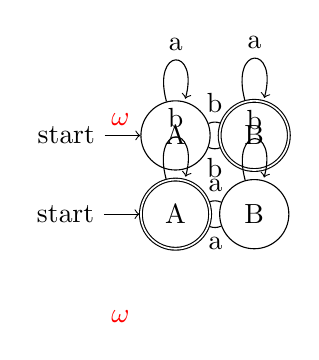
\begin{tikzpicture}
        \node[align=center, text=red] at (-0.7, 0.2) {{$\omega$}};
        \node[align=center, text=red] at (-0.7, -2.3) {{$\omega$}};
        \node[state, initial] (0) {A};
        \node[state, accepting, right of=0] (1) {B};
        \node[state, below of=1] (2) {B};
        \node[state, initial, accepting, left of=2] (3) {A};
        \draw (0) edge[above, bend left=20] node{b} (1)
        (0) edge[loop above] node{a} (0)
        (1) edge[below, bend left=20] node{b} (0)
        (1) edge[loop above] node{a} (1)
        (2) edge[below, bend left=20] node{a} (3)
        (2) edge[loop above] node{b} (2)
        (3) edge[above, bend left=20] node{a} (2)
        (3) edge[loop above] node{b} (3)
        ;
    \end{tikzpicture}
\end{document}
